\section{Лекция 1 - 01.09.2020 - Ряды}
\subsection{Определение ряда}
\begin{definition}
Пусть $a_{n}$ -- последовательность, т.е. $\NN \rightarrow \RR$. Формальная бесконечная сумма: $a_1 + a_2 + a_3 + \dots = \sum_{n=1}^{\infty} a_n$ называется рядом.
$S_N = \sum_{n = 1}^{N} a_n$ -- частичная сумма, сумма ряда: $S = \lim_{N \rightarrow \infty} S_N$
\end{definition}

Возможны 3 случая:
\begin{enumerate}
    \item $\exists S \in \RR$
    \item $\exists S = \infty$
    \item $\nexists S$
\end{enumerate}

В первом случае говорят, что ряд сходится, иначе -- что рял расходится.

\begin{example}~
    \begin{enumerate}
        \item $\sum_{n = 1}^{\infty} 0 = 0 + 0 + \dots + 0 = 0$
        \item $\sum_{n = 1}^{\infty} 1 = 1 + 1 + \dots + 1 = \infty$
        \item $\sum_{n = 1}^{\infty} (-1)^{n} = -1 + 1 - \dots$ не существует
    \end{enumerate}
\end{example}

\begin{definition}
    Если ряд сходится, т.е. $S_N \rightarrow S$ при $N \rightarrow \infty$, то $S - S_N = r_N$ -- остаток ряда

    $r_N = \sum_{n = N + 1}^{\infty} a_n$, $r_N \rightarrow 0$ при $N \rightarrow \infty$
\end{definition}

\subsection{Необходимое условие сходимости}
\begin{comment}~
    Если ряд сходится, то $a_n \rightarrow 0$
\end{comment}
\begin{proof}
    $a_n = S_n - S_{n - 1} \rightarrow 0$, т.к. $S_n \rightarrow S$ и $S_{n - 1} \rightarrow S$
\end{proof}
\subsection{Критерий Коши}
\begin{definition}
    ${a_n}$ называется фундаментальной, если $\forall \epsilon > 0$  $\exists N: \forall n > m > N \implies |S_n - S_m| < \epsilon$
\end{definition}
\begin{theorem}
    ${S_n}$ -- сходится $\Leftrightarrow {S_n}$ -- фундаментальная
\end{theorem}
\begin{proof}
$S_n - S_m = \sum_{k = m + 1}^{n} a_{k}$
Тогда $\sum a_n$ -- сходится $\Leftrightarrow$ $\forall \epsilon > 0$  $\exists N: \forall n > m > N$
$|a_{m + 1} + a_{m + 2} + \dots + a_{n}| < \epsilon$
\end{proof}

\begin{example}~
\begin{enumerate}
    \item $\sum_{n = 1}^{\infty} \dfrac{1}{n(n + 1)}$
    
    Заметим, что $S_N = \sum_{n = 1}^{N} \dfrac{1}{n(n + 1)} = \sum_{n = 1}^{N}$
    $\left(\dfrac{1}{n} - \dfrac{1}{n + 1}\right) = \left(1 - \dfrac{1}{2}\right) + \left(\dfrac{1}{2} - \dfrac{1}{3}\right) + \dots + \left(\dfrac{1}{N} - \dfrac{1}{N + 1}\right) = 1 - \dfrac{1}{N + 1} \rightarrow 1$

    Этот ряд сходится при $N \to \infty$: $\sum_{n = 1}^{\infty} \dfrac{1}{n(n + 1)} = 1$

    \item $z \in \CC$, $z = |z| \cdot (\cos \varphi + i \sin \varphi)$
    
    \tikzset{every picture/.style={line width=0.75pt}} %set default line width to 0.75pt        
    
    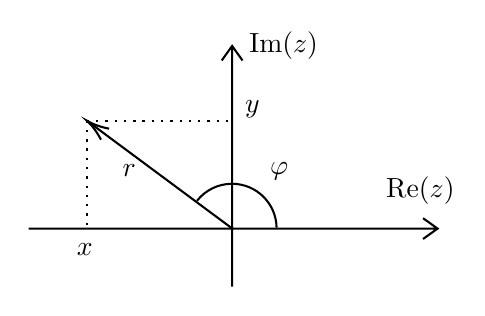
\begin{tikzpicture}[x=0.75pt,y=0.75pt,yscale=-1,xscale=1]
    %uncomment if require: \path (0,300); %set diagram left start at 0, and has height of 300
    
    %Shape: Axis 2D [id:dp5021355999575146] 
    \draw  (146.24,121.3) -- (343.24,121.3)(244.24,33.3) -- (244.24,149.3) (336.24,116.3) -- (343.24,121.3) -- (336.24,126.3) (239.24,40.3) -- (244.24,33.3) -- (249.24,40.3)  ;
    %Straight Lines [id:da816813378460219] 
    \draw    (244.19,121.19) -- (175.85,70.49) ;
    \draw [shift={(174.24,69.3)}, rotate = 396.57] [color={rgb, 255:red, 0; green, 0; blue, 0 }  ][line width=0.75]    (10.93,-3.29) .. controls (6.95,-1.4) and (3.31,-0.3) .. (0,0) .. controls (3.31,0.3) and (6.95,1.4) .. (10.93,3.29)   ;
    %Straight Lines [id:da3059124343527635] 
    \draw  [dash pattern={on 0.84pt off 2.51pt}]  (174.24,69.3) -- (174.24,121.3) ;
    %Straight Lines [id:da7341650820111749] 
    \draw  [dash pattern={on 0.84pt off 2.51pt}]  (174.24,69.3) -- (244.24,69.3) ;
    %Shape: Arc [id:dp4110961564541693] 
    \draw  [draw opacity=0] (227.31,107.92) .. controls (231.24,102.92) and (237.34,99.71) .. (244.19,99.71) .. controls (255.91,99.71) and (265.44,109.11) .. (265.66,120.79) -- (244.19,121.19) -- cycle ; \draw   (227.31,107.92) .. controls (231.24,102.92) and (237.34,99.71) .. (244.19,99.71) .. controls (255.91,99.71) and (265.44,109.11) .. (265.66,120.79) ;
    
    % Text Node
    \draw (168,127) node [anchor=north west][inner sep=0.75pt]   [align=left] {$\displaystyle x$};
    % Text Node
    \draw (249,58) node [anchor=north west][inner sep=0.75pt]   [align=left] {$\displaystyle y$};
    % Text Node
    \draw (190,89) node [anchor=north west][inner sep=0.75pt]   [align=left] {$\displaystyle r$};
    % Text Node
    \draw (261,88) node [anchor=north west][inner sep=0.75pt]   [align=left] {$\displaystyle \varphi $};
    % Text Node
    \draw (317,95) node [anchor=north west][inner sep=0.75pt]   [align=left] {Re$\displaystyle ( z)$};
    % Text Node
    \draw (251,25) node [anchor=north west][inner sep=0.75pt]   [align=left] {Im$\displaystyle ( z)$};
    
    
    \end{tikzpicture}
    
    Рассмотрим ряд $\sum_{n = 0}^{\infty} z^n = 1 + z + z ^ 2 + \dots$
    

    $S_N = 1 + z + z^2 + \dots + z^N = \dfrac{1 - z^{N + 1}}{1 - z}$

    Ряд сходится $\Leftrightarrow |z| < 1$
    
    $|z| < 1 \Rightarrow z^n \rightarrow 0$, $S_N = \dfrac{1 - z^{N + 1}}{1 - z} \to \dfrac{1}{1 - z}$ 
\end{enumerate}
\end{example}
\subsection{Положительные ряды}
$\sum_{n = 1}^{\infty} a_n, a_n \geq 0$, 
$S_n \uparrow$, т.к. $S_{n + 1} \geq S_{n}$

Возможны 2 случая:
\begin{enumerate}
    \item $\exists S \in \RR$
    \item $\exists S = \infty$
\end{enumerate}
\begin{designation}
    $\sum_{n = 1}^{\infty} a_n < \infty$ -- ряд сходится,
    $\sum_{n = 1}^{\infty} a_n = \infty$ -- ряд расходится.
\end{designation}
\subsection{Признаки сравнения}
	\begin{enumerate}
	\item Сравнение с помощью неравенства.
	
	$a_n \leqslant b_n$ при всех $n \geqslant n_0$
	
	Ряд $\sum b_n$ cходится $\implies$ ряд $\sum a_n$ сходится
	
	Ряд $\sum a_n$ расходится $\implies$ ряд $\sum b_n$ расходится
	
	
	\item Сравнение отношений.
	
	$\frac{a_{n+1}}{a_n} \leqslant \frac{b_{n+1}}{b_n}$ при всех $n \geqslant n_0$
	
	Ряд $\sum b_n$ cходится $\implies$ ряд $\sum a_n$ сходится
	
	Ряд $\sum a_n$ расходится $\implies$ ряд $\sum b_n$ расходится
	
	\begin{proof}~
	
	$a_{n_0+1} \leqslant \frac{a_{n_0}}{b_{n_0}}\cdot b_{n_0 + 1}$
	
	$a_{n_0+2} \leqslant \frac{a_{n_0 + 1}}{b_{n_0 + 1}}\cdot b_{n_0 + 2} \leqslant \frac{a_{n_0}}{b_{n_0}}\cdot b_{n_0 + 2}$
	
	$\vdots$
	
	$a_{n_0+k} \leqslant \frac{a_{n_0}}{b_{n_0}}\cdot b_{n_0 + k} \implies \sum_{n=n_0}^{N} a_n \leqslant \frac{a_{n_0}}{b_{n_0}}\cdot \sum_{n=n_0}^{N} b_n$
	\end{proof}

	\item Сравнение с помощью предела.
	
	$\lim_{n \to \infty} \frac{a_n}{b_n} \in (0; +\infty) \implies$ сходимость $\sum a_n \iff$ сходимость $\sum b_n$
	
	\begin{proof}~
		
	$c = \lim_{n \to \infty} \frac{a_n}{b_n} > 0$
	
	$\forall \epsilon\ \exists n_0:\ c - \epsilon \leqslant \frac{a_n}{b_n} \leqslant c + \epsilon$, $\forall n \geqslant n_0$
	
	Возьмём $\epsilon : c - \epsilon > 0 \implies (c - \epsilon)\cdot b_n \leqslant a_n \leqslant (c + \epsilon)\cdot b_n$
	
	Сходимость следует из правой части неравенства, а расходимость из левой. 
	\end{proof}
\end{enumerate}
\subsection{Отсутствие универсального ряда сравнения}
	\begin{proposal}
	Не существует ряда $\sum c_n,\ c_n > 0:$ 
	
	1) $\frac{a_n}{c_n} \to 0 \implies$ ряд $\sum a_n$ сходится.
	
	2) $\frac{b_n}{c_n} \to \infty \implies$ ряд $\sum b_n$ расходится.
\end{proposal}

\begin{proof}~
	
	\begin{enumerate}
		\item Если ряд $\sum c_n$ расходится, то пусть $S_N = \sum_{n=1}^{N} c_n \to \infty, S_0=0$, тогда ряд $\sum_{n=1}^{\infty} (\underbrace{\sqrt{S_n} - \sqrt{S_{n - 1}}}_{a_n})$ расходится так как:
		
		\begin{enumerate}
			\item $\sum_{n=1}^{N} (\sqrt{S_n} - \sqrt{S_{n-1}}) = \sqrt{S_1} - \sqrt{S_0} + \sqrt{S_2} - \sqrt{S_1} + \dots + \sqrt{S_N} - \sqrt{S_{N-1}} = \sqrt{S_N} - \sqrt{S_0} = \sqrt{S_N} \to \sqrt{S}$
			
			\item $\frac{\sqrt{S_n} - \sqrt{S_{n-1}}}{c_n} = \frac{\sqrt{S_n} - \sqrt{S_{n-1}}}{S_n - S_{n - 1}} = \frac{1}{\sqrt{S_n} + \sqrt{S_{n - 1}}} \implies \frac{a_n}{c_n} \to 0$
		\end{enumerate}
		
		Ряд расходится, но по предположению сходится, получили противоречие.
		
		\item Если ряд $\sum_{n=1}^{\infty} c_n$ сходится, то рассмотрим $r_n$ - его $n$-ный остаток, тогда ряд $\sum_{n=1}^{\infty} (\underbrace{\sqrt{r_{n-1}} - \sqrt{r_n}}_{b_n})$, $r_0 = S = \sum_{n = 1}^{\infty} c_n$ сходится, так как:
		
		\begin{enumerate}
			\item $\sum_{n=1}^{N} (\sqrt{r_{n-1}} - \sqrt{r_n}) = \sqrt{r_0} - \sqrt{r_1} + \sqrt{r_1} - \sqrt{r_2} + \dots + \sqrt{r_{N-1}} - \sqrt{r_{N}}= \sqrt{r_0} - \sqrt{r_N} = \sqrt{S} - \sqrt{r_N} \to \sqrt{S}$, т.к. $r_N \to 0$
			
			\item $\frac{\sqrt{r_{n-1}} - \sqrt{r_n}}{c_n} = \frac{\sqrt{r_{n-1}} - \sqrt{r_n}}{r_{n-1} - r_n} = \frac{1}{\sqrt{r_{n-1}} + \sqrt{r_n}} \to \infty$, т.к. $\sqrt{r_{n-1}} \to 0$ и $\sqrt{r_n} \to 0$
		\end{enumerate}
		
        Ряд сходится, но по предположению расходится, получили противоречие.
	\end{enumerate}
\end{proof}